
%%%
% Regularization to prevent too strong of weights
%%%

\subsubsection*{Regularization}

%%%
% Process
%%%

%%%
As an attempt to prevent a single strategy's weight from being so strongly 
preferred that a second strategy could not hope to possibly gain ground,
a hard limit was placed on the pre-normalized update value.
%
Expressed mathematically,
\[
    \wvecm'_{p,o,d}[i] = \max\{K,c\wvecm_{p,o,d}[i]\}
\]
where $K$ is some constant value throughout the training.
%
While the value of $w_{m,o,d}[i]$ could exceed $K$ after re-normalization
for a particularly strongly weighted strategy,
the value could be seen converging to $K$ within just a handful of iterations.
%
The desired intention of this regularization was to allow other strategies
the opportunity to overcome the bias of earlier strengthening of the strongest
strategy.
%%%

\paragraph*{Results}

%%%
% Results:
%	Similar areas taken up for hand_max_{min,avg}
%		both share same space rather than Croatia/Boz&Herz-shape
%	Grayer, since values only so large
%	As max value is increased,
%		darker, more like un-regulated
%	Islands still present
%	losing, still uncertain
%		still chance of higher than regulation, because of aforementioned reason
%%%


\begin{figure}
\center

	\begin{subfigure}[t]{0.22\textwidth}
		\center
		
\includegraphics[width=\textwidth]{images/findings/experiments/regularization/strats/0.50/hand_max_min.png}
		\caption{\handmaxmin}
	\end{subfigure}
	~
	\begin{subfigure}[t]{0.22\textwidth}
		\center
		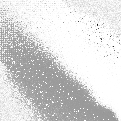
\includegraphics[width=\textwidth]{images/findings/experiments/regularization/strats/0.50/hand_max_avg.png}
		\caption{\handmaxavg}
	\end{subfigure}
~
	\begin{subfigure}[t]{0.22\textwidth}
		\center
		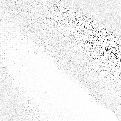
\includegraphics[width=\textwidth]{images/findings/experiments/regularization/strats/0.50/hand_max_med.png}
		\caption{\handmaxmed}
	\end{subfigure}
	~
	\begin{subfigure}[t]{0.22\textwidth}
		\center
		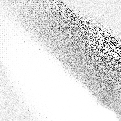
\includegraphics[width=\textwidth]{images/findings/experiments/regularization/strats/0.50/hand_max_poss.png}
		\caption{\handmaxposs}
	\end{subfigure}

	\begin{subfigure}[t]{0.22\textwidth}
		\center
		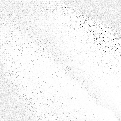
\includegraphics[width=\textwidth]{images/findings/experiments/regularization/strats/0.50/crib_min_avg.png}
		\caption{\cribminavg}
	\end{subfigure}
	~
	\begin{subfigure}[t]{0.22\textwidth}
		\center
		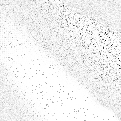
\includegraphics[width=\textwidth]{images/findings/experiments/regularization/strats/0.50/pegging_max_avg_gained.png}
		\caption{\peggingmaxavggained}
	\end{subfigure}
~
	\begin{subfigure}[t]{0.22\textwidth}
		\center
		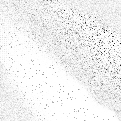
\includegraphics[width=\textwidth]{images/findings/experiments/regularization/strats/0.50/pegging_max_med_gained.png}
		\caption{\peggingmaxmedgained}
	\end{subfigure}
	~
	\begin{subfigure}[t]{0.22\textwidth}
		\center
		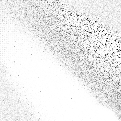
\includegraphics[width=\textwidth]{images/findings/experiments/regularization/strats/0.50/pegging_min_avg_given.png}
		\caption{\peggingminavggiven}
	\end{subfigure}

\caption{
	Final strategies for an agent using regularized learning
	when playing as the pone
	and the maximum value weight allowed is 0.50
	after training for 500,000 games.
}
\label{fig:reg-strats-0.50}
\end{figure}

%
\begin{figure}
\center

	\begin{subfigure}[t]{0.22\textwidth}
		\center
		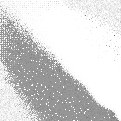
\includegraphics[width=\textwidth]{images/findings/experiments/regularization/strats/0.60/hand_max_min.png}
		\caption{\handmaxmin}
	\end{subfigure}
	~
	\begin{subfigure}[t]{0.22\textwidth}
		\center
		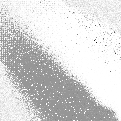
\includegraphics[width=\textwidth]{images/findings/experiments/regularization/strats/0.60/hand_max_avg.png}
		\caption{\handmaxavg}
	\end{subfigure}
~
	\begin{subfigure}[t]{0.22\textwidth}
		\center
		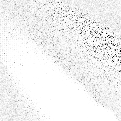
\includegraphics[width=\textwidth]{images/findings/experiments/regularization/strats/0.60/hand_max_med.png}
		\caption{\handmaxmed}
	\end{subfigure}
	~
	\begin{subfigure}[t]{0.22\textwidth}
		\center
		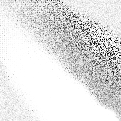
\includegraphics[width=\textwidth]{images/findings/experiments/regularization/strats/0.60/hand_max_poss.png}
		\caption{\handmaxposs}
	\end{subfigure}

	\begin{subfigure}[t]{0.22\textwidth}
		\center
		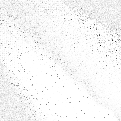
\includegraphics[width=\textwidth]{images/findings/experiments/regularization/strats/0.60/crib_min_avg.png}
		\caption{\cribminavg}
	\end{subfigure}
	~
	\begin{subfigure}[t]{0.22\textwidth}
		\center
		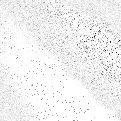
\includegraphics[width=\textwidth]{images/findings/experiments/regularization/strats/0.60/pegging_max_avg_gained.png}
		\caption{\peggingmaxavggained}
	\end{subfigure}
~
	\begin{subfigure}[t]{0.22\textwidth}
		\center
		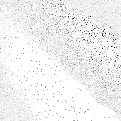
\includegraphics[width=\textwidth]{images/findings/experiments/regularization/strats/0.60/pegging_max_med_gained.png}
		\caption{\peggingmaxmedgained}
	\end{subfigure}
	~
	\begin{subfigure}[t]{0.22\textwidth}
		\center
		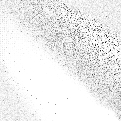
\includegraphics[width=\textwidth]{images/findings/experiments/regularization/strats/0.60/pegging_min_avg_given.png}
		\caption{\peggingminavggiven}
	\end{subfigure}

\caption{
	Final strategies for an agent using regularized learning
	when playing as the dealer
	and the maximum value weight allowed is 0.60
	after training for 500,000 games.
}
\label{fig:neighbor-strats}
\end{figure}

%
\begin{figure}
\center

	\begin{subfigure}[t]{0.22\textwidth}
		\center
		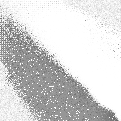
\includegraphics[width=\textwidth]{images/findings/experiments/regularization/strats/0.70/hand_max_min.png}
		\caption{\handmaxmin}
	\end{subfigure}
	~
	\begin{subfigure}[t]{0.22\textwidth}
		\center
		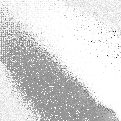
\includegraphics[width=\textwidth]{images/findings/experiments/regularization/strats/0.70/hand_max_avg.png}
		\caption{\handmaxavg}
	\end{subfigure}
~
	\begin{subfigure}[t]{0.22\textwidth}
		\center
		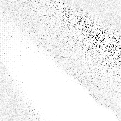
\includegraphics[width=\textwidth]{images/findings/experiments/regularization/strats/0.70/hand_max_med.png}
		\caption{\handmaxmed}
	\end{subfigure}
	~
	\begin{subfigure}[t]{0.22\textwidth}
		\center
		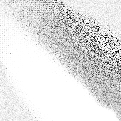
\includegraphics[width=\textwidth]{images/findings/experiments/regularization/strats/0.70/hand_max_poss.png}
		\caption{\handmaxposs}
	\end{subfigure}

	\begin{subfigure}[t]{0.22\textwidth}
		\center
		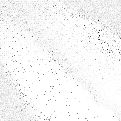
\includegraphics[width=\textwidth]{images/findings/experiments/regularization/strats/0.70/crib_min_avg.png}
		\caption{\cribminavg}
	\end{subfigure}
	~
	\begin{subfigure}[t]{0.22\textwidth}
		\center
		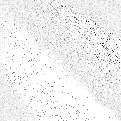
\includegraphics[width=\textwidth]{images/findings/experiments/regularization/strats/0.70/pegging_max_avg_gained.png}
		\caption{\peggingmaxavggained}
	\end{subfigure}
~
	\begin{subfigure}[t]{0.22\textwidth}
		\center
		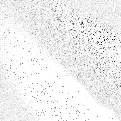
\includegraphics[width=\textwidth]{images/findings/experiments/regularization/strats/0.70/pegging_max_med_gained.png}
		\caption{\peggingmaxmedgained}
	\end{subfigure}
	~
	\begin{subfigure}[t]{0.22\textwidth}
		\center
		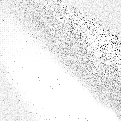
\includegraphics[width=\textwidth]{images/findings/experiments/regularization/strats/0.70/pegging_min_avg_given.png}
		\caption{\peggingminavggiven}
	\end{subfigure}

\caption{
	Final strategies for an agent using regularized learning
	when playing as the pone
	and the maximum value weight allowed is 0.70
	after training for 500,000 games.
}
\label{fig:reg-strats-0.70}
\end{figure}


\begin{figure}
\center

	\begin{subfigure}[t]{0.22\textwidth}
		\center
		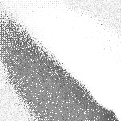
\includegraphics[width=\textwidth]{images/findings/experiments/regularization/strats/0.80/hand_max_min.png}
		\caption{\handmaxmin}
	\end{subfigure}
	~
	\begin{subfigure}[t]{0.22\textwidth}
		\center
		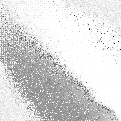
\includegraphics[width=\textwidth]{images/findings/experiments/regularization/strats/0.80/hand_max_avg.png}
		\caption{\handmaxavg}
	\end{subfigure}
~
	\begin{subfigure}[t]{0.22\textwidth}
		\center
		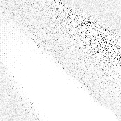
\includegraphics[width=\textwidth]{images/findings/experiments/regularization/strats/0.80/hand_max_med.png}
		\caption{\handmaxmed}
	\end{subfigure}
	~
	\begin{subfigure}[t]{0.22\textwidth}
		\center
		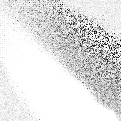
\includegraphics[width=\textwidth]{images/findings/experiments/regularization/strats/0.80/hand_max_poss.png}
		\caption{\handmaxposs}
	\end{subfigure}

	\begin{subfigure}[t]{0.22\textwidth}
		\center
		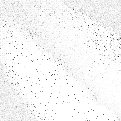
\includegraphics[width=\textwidth]{images/findings/experiments/regularization/strats/0.80/crib_min_avg.png}
		\caption{\cribminavg}
	\end{subfigure}
	~
	\begin{subfigure}[t]{0.22\textwidth}
		\center
		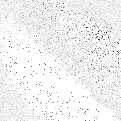
\includegraphics[width=\textwidth]{images/findings/experiments/regularization/strats/0.80/pegging_max_avg_gained.png}
		\caption{\peggingmaxavggained}
	\end{subfigure}
~
	\begin{subfigure}[t]{0.22\textwidth}
		\center
		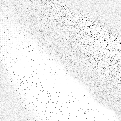
\includegraphics[width=\textwidth]{images/findings/experiments/regularization/strats/0.80/pegging_max_med_gained.png}
		\caption{\peggingmaxmedgained}
	\end{subfigure}
	~
	\begin{subfigure}[t]{0.22\textwidth}
		\center
		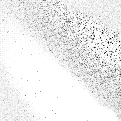
\includegraphics[width=\textwidth]{images/findings/experiments/regularization/strats/0.80/pegging_min_avg_given.png}
		\caption{\peggingminavggiven}
	\end{subfigure}

\caption{
	Final strategies for an agent using regularized learning
	when playing as the dealer
	and the maximum value weight allowed is 0.80
	after training for 500,000 games.
}
\label{fig:reg-strats-0.80}
\end{figure}


\begin{figure}
\centering

	\begin{tabular}{l l p{2.75cm} p{2.75cm} p{2.75cm} p{2.75cm}}
	& & \multicolumn{4}{c}{\textit{Regularization Rate}} \\
	&
		& $r = 0.5$
		& $r = 0.6$
		& $r = 0.7$
		& $r = 0.8$
		\\
	%
	\multirow{2}{*}{
	\rotatebox{90}{
	\parbox[c]{2.5cm}{
		\textit{Strategy}
	}
	}
	}
	%
	& \rotatebox[origin=c]{90}{\handmaxmin}
		&\parbox[c]{1em}{
\includegraphics[width=\stratgraphwidthmed]{images/findings/experiments/regularization/strats/0.50/hand_max_min.png}}
		&\parbox[c]{1em}{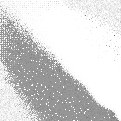
\includegraphics[width=\stratgraphwidthmed]{images/findings/experiments/regularization/strats/0.60/hand_max_min.png}}
		&\parbox[c]{1em}{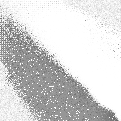
\includegraphics[width=\stratgraphwidthmed]{images/findings/experiments/regularization/strats/0.70/hand_max_min.png}}
		&\parbox[c]{1em}{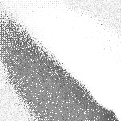
\includegraphics[width=\stratgraphwidthmed]{images/findings/experiments/regularization/strats/0.80/hand_max_min.png}}
	%
	\\ & & & & & \\
	& \rotatebox[origin=c]{90}{\handmaxavg}
		&\parbox[c]{1em}{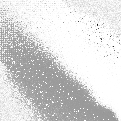
\includegraphics[width=\stratgraphwidthmed]{images/findings/experiments/regularization/strats/0.50/hand_max_avg.png}}
		&\parbox[c]{1em}{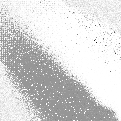
\includegraphics[width=\stratgraphwidthmed]{images/findings/experiments/regularization/strats/0.60/hand_max_avg.png}}
		&\parbox[c]{1em}{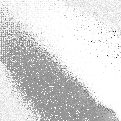
\includegraphics[width=\stratgraphwidthmed]{images/findings/experiments/regularization/strats/0.70/hand_max_avg.png}}
		&\parbox[c]{1em}{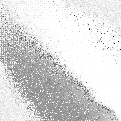
\includegraphics[width=\stratgraphwidthmed]{images/findings/experiments/regularization/strats/0.80/hand_max_avg.png}}
\end{tabular}

\caption{
	Comparison of the \handmaxmin\ and \handmaxavg\ strategies
	for each of the regularization rates ($r$) used
	when the agent is playing as the pone.
}
\label{fig:expts-reg-comp}
\end{figure}



%%%
As was expected,
the limitation of maximum attainable value did indeed force the agent to learn
multiple applicable strategies for each score location.
%
As can be seen in Figure~\ref{fig:reg-strats-0.50},
the \handmaxmin\ and \handmaxavg\ strategies are now 
more or less equally represented across the winning triangle area.
%
This is demonstrated by the monotone gray seen in these locations.
%
Rather than each strategy specializing to its own dominant location,
the territory is shared between the two most applicable strategies.
%
Therefore,
the regularization does indeed prevent the dominance of a single strategy
unintentionally discarding all other potential strategies.
%%%

%%%
Additionally,
the nature of this gray mass alters significantly as the regularization rate is
altered.
%
With a lower allowed maximum value,
the strategy graphs take on the previously mentioned slightly amorphous gray
blob shape.
%
As the maximum value approaches one,
the gray shape begins to specialize more and begins to show resemblance to the
final strategy graphs obtained without regularization.
%
A visualization of this process can be found in
Figure~\ref{fig:expts-reg-comp}.
%%%


\begin{figure}

	\begin{subfigure}[t]{0.48\textwidth}
		\center
		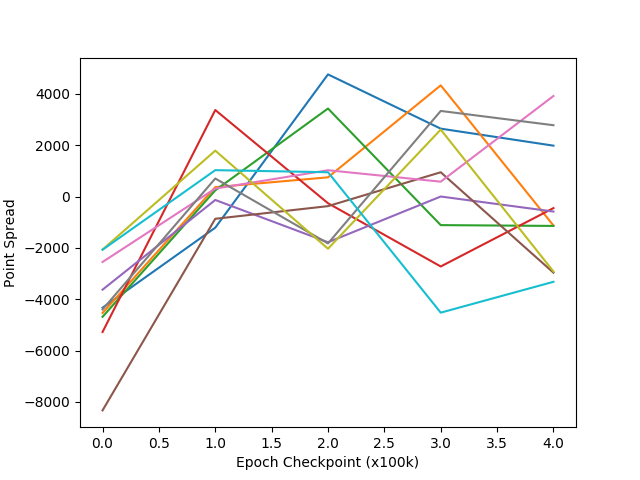
\includegraphics[width=\textwidth]{images/findings/experiments/regularization/tourny/reg_050-kyttuhat-strict-500k.png}
		\caption{$r = 0.50$}
	\end{subfigure}
	~
	\begin{subfigure}[t]{0.48\textwidth}
		\center
		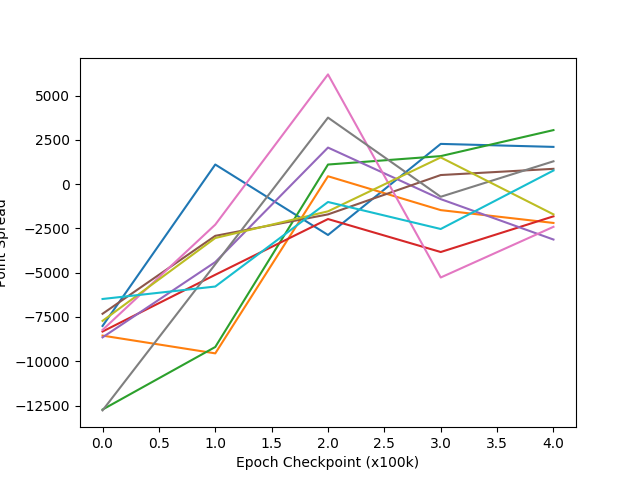
\includegraphics[width=\textwidth]{images/findings/experiments/regularization/tourny/reg_060-kyttuhat-strict-500k.png}
		\caption{$r = 0.60$}
	\end{subfigure}

	\begin{subfigure}[t]{0.48\textwidth}
		\center
		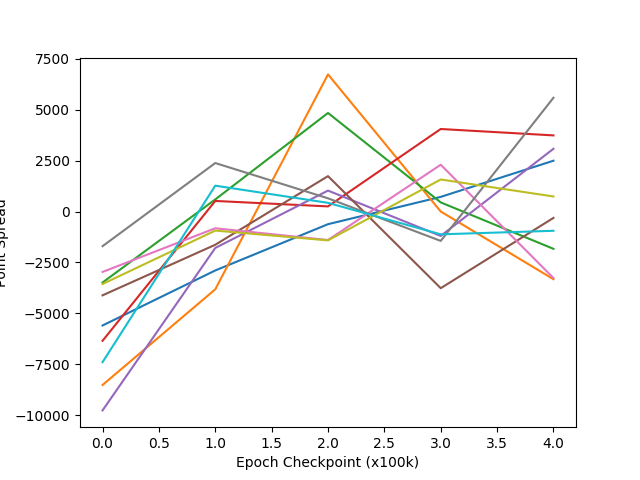
\includegraphics[width=\textwidth]{images/findings/experiments/regularization/tourny/reg_070-kyttuhat-strict-500k.png}
		\caption{$r = 0.70$}
	\end{subfigure}
	~
	\begin{subfigure}[t]{0.48\textwidth}
		\center
		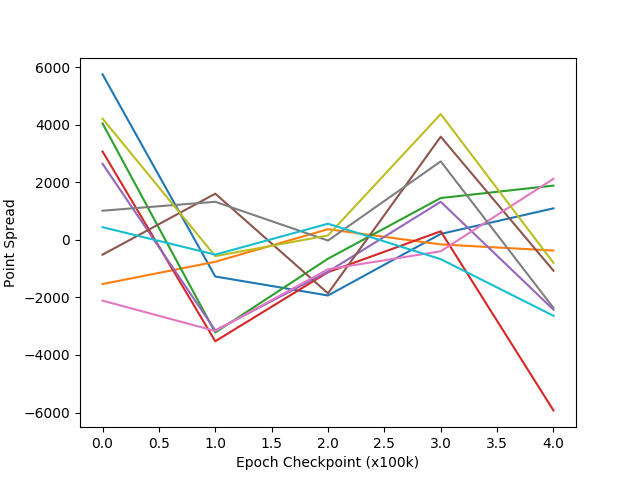
\includegraphics[width=\textwidth]{images/findings/experiments/regularization/tourny/reg_080-kyttuhat-strict-500k.png}
		\caption{$r = 0.80$}
	\end{subfigure}

\caption{
	Point spreads of self-tournaments for 10,000 games
	carried out between agents trained using
	the regulation method mentioned in Section~\ref{sec:findings-r2} after being
	trained for 500,000 games.
	Each tournament plot in n this figure is referenced by the regularization
	rate $r$ in use during training.
}
\label{fig:reg-tournies}
\end{figure}


%%%
Furthermore,
as can be seen in Figure~\ref{fig:reg-tournies},
only a regularization rate of $r = 0.80$ (Figure~\ref{fig:reg-tournies-0.80}
can be said to be similar to a loss curve.
%
With rates of $r=0.50$ (Figure~\ref{fig:reg-tournies-0.50},
$r = 0.60$ (Figure~\ref{fig:reg-tournies-0.60}),
and $r = 0.70$ (Figure~\ref{fig:reg-tournies-0.70}),
the tournament point spread curves show that a trained agent plays on par with
its recent checkpoints,
but consistently worse than random weights.
%
The endpoints of the point spread curves using $r = 0.80$
show a decrease from better-than-random play for the trained agent
to more-or-less on-par performance with its later checkpoints,
indicative of an increase in performance as training progresses.
%
However,
the increases and decreases of performance along the time axis,
the wide range of spreads present,
and the sinusoidal nature of intermediate checkpoints' spreads
prevents the conclusion that performance is as predictable as that.
%%%

